% -----------------------------------------------------------------
% Document class: Article
\documentclass[ a4paper, twoside, 11pt]{article}
\usepackage{../../macros-general}
\usepackage{../../macros-article}
%\graphicspath{{./figures/}}
% Number of the handout, quiz, exam, etc.
\newcommand{\numero}{03}
\setcounter{numero}{\numero}

% -----------------------------------------------------------------
\begin{document}
\allowdisplaybreaks

% Indices
\newcommand{\iava}{$i$\tsup{ava} }
\newcommand{\iavo}{$i$\tsup{avo} }
\newcommand{\java}{$j$\tsup{ava} }
\newcommand{\javo}{$j$\tsup{avo} }
\newcommand{\kava}{$k$\tsup{ava} }
\newcommand{\kavo}{$k$\tsup{avo} }
\newcommand{\tava}{$t$\tsup{ava} }
\newcommand{\tavo}{$t$\tsup{avo} }
\newcommand{\tmava}{$(t-1)$\tsup{ava} }
\newcommand{\tmavo}{$(t-1)$\tsup{avo} }
\newcommand{\tMava}{$(t+1)$\tsup{ava} }
\newcommand{\tMavo}{$(t+1)$\tsup{avo} }

\begin{center}
\Large Modelos Estoc\'asticos (INDG-1008): Lecci\'on \numero \\[2ex]
\small \textbf{Semestre:} 2017-2018 T\'ermino II \qquad
\textbf{Instructor:} Luis I. Reyes Castro
\end{center}
\fullskip

% -----------------------------------------------------------------
\begin{problem}
El aeropuerto internacional de Centerville tiene dos pistas, una solo para despegues y otra solo para aterrizajes. Los aviones llegan al espacio a\'ereo del aeropuerto, el cual tiene una capacidad para $C = 7$ aeronaves, para pedir instrucciones de aterrizaje seg\'un un proceso de Poisson con tasa media de $\lambda$ por hora. El tiempo que se requiere para realizar un aterrizaje despu\'es de la aprobaci\'on tiene distribuci\'on exponencial con media de 3 minutos, proceso que debe estar terminado antes de aprobar otro aterrizaje. Los aviones en espera de pista vuelan en c\'irculos. 

La FAA (Administraci\'on de Aviaci\'on Federal, por sus siglas en ing\'es) tiene varios criterios respecto del nivel seguro de congesti\'on de aviones en espera para aterrizar. Estos criterios dependen de varios factores en cada aeropuerto, como el n\'umero de pistas disponibles. En el caso de Centerville los criterios son \textit{(i)} el n\'umero promedio de aviones en espera no debe exceder de 1, \textit{(ii)} el 95\% del tiempo, el n\'umero real de aviones en espera no debe exceder de 4, y \textit{(iii)} para el 99\% de los aviones, el tiempo que vuelan en c\'irculos antes de aterrizar no debe exceder de 30 minutos. 

Complete las siguientes actividades: 
\begin{enumerate}[label=\textbf{\alph*)}]
\item \textbf{2 Puntos:} Calcule la distribuci\'on estacionaria del sistema para los casos cuando la tasa de arribo es de $\lambda = 10$ por hora, $\lambda = 15$ por hora, y $\lambda = 25$ por hora. 

\emph{Soluci\'on:} Primero reconocemos que como solo hay una pista de aterrizaje, este problema corresponde a un modelo M/M/1/7 cuya tasa de servicio por pista es de $\mu = 20$ aeronaves por hora. Luego podemos bosquejar la Cadena de Markov correspondiente, tal como se muestra en la siguiente fotograf\'ia. 

\begin{figure}[htb]
\centering
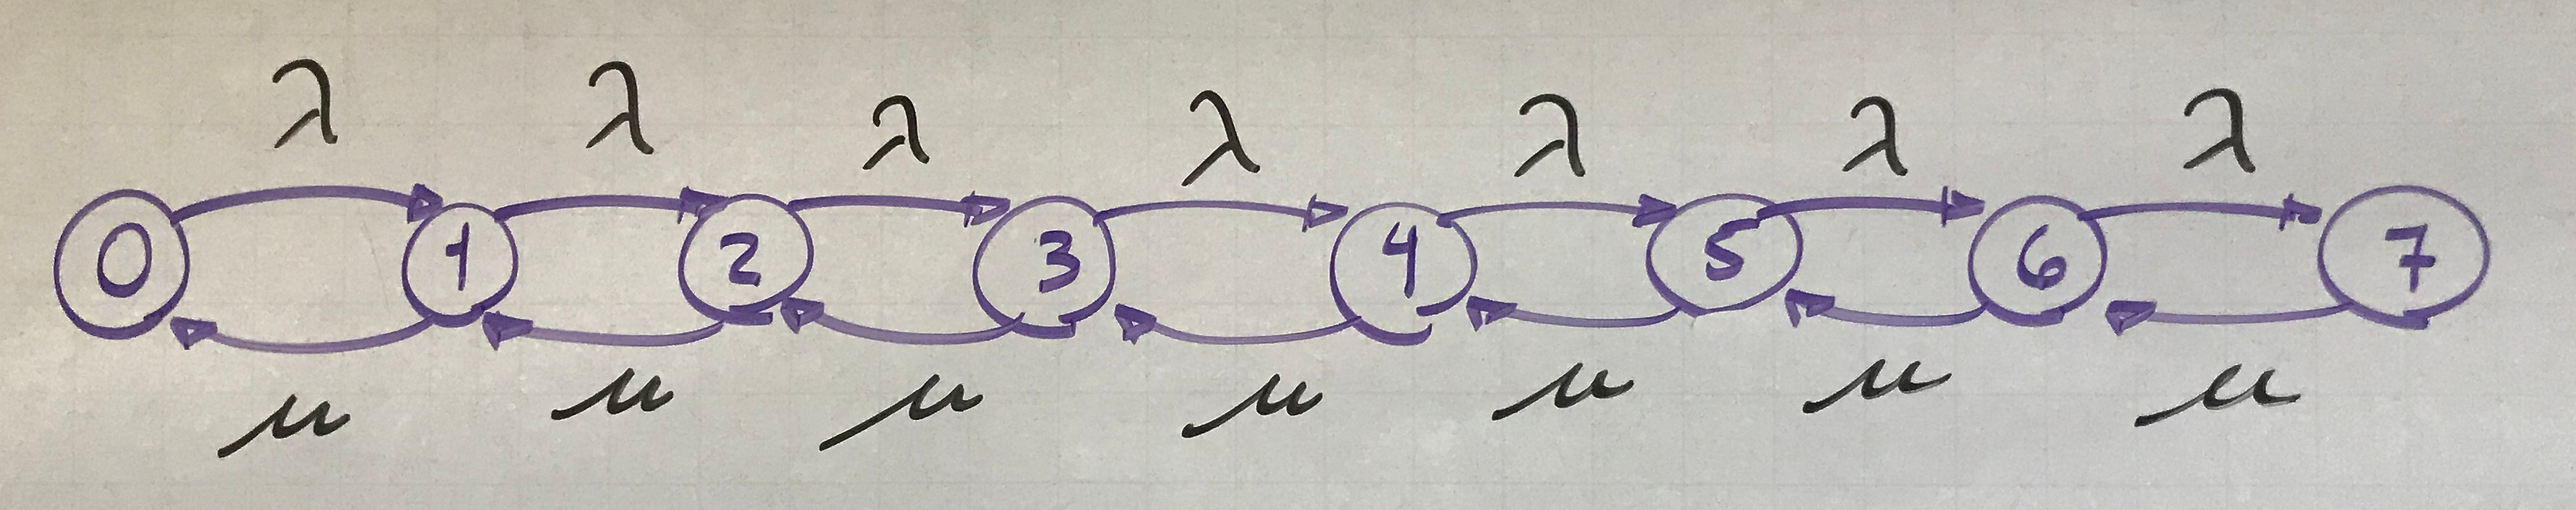
\includegraphics[width=0.8\textwidth]{problema-1-A.jpg}
\end{figure}

Para esta cadena, definiendo $\rho \define \lambda / \mu$, tenemos: 
\begin{align*}
& \lambda = 10 \quad \Longrightarrow \quad \rho = 0.50 \\
& \lambda = 15 \quad \Longrightarrow \quad \rho = 0.75 \\
& \lambda = 25 \quad \Longrightarrow \quad \rho = 1.25
\end{align*}
Las ecuaciones de balance son: 
\begin{align*}
& E_0 \; \colon \; \lambda \, \pi_0 \; = \; \mu \, \pi_1
\quad \Longrightarrow \quad
\pi_1 \; = \; \rho \, \pi_0 \\
& E_1 \; \colon \; (\lambda + \mu) \, \pi_1
\; = \; \lambda \, \pi_0 + \mu \, \pi_2
\quad \Longrightarrow \quad
\pi_2 \; = \; \rho^2 \, \pi_0 \\
& E_2 \; \colon \; (\lambda + \mu) \, \pi_2
\; = \; \lambda \, \pi_1 + \mu \, \pi_3
\quad \Longrightarrow \quad
\pi_3 \; = \; \rho^3 \, \pi_0 \\
& \vdots \\
& E_k \; \colon \; (\lambda + \mu) \, \pi_{k} \; = \; \lambda \, \pi_{k-1} + \mu \, \pi_{k+1} \quad \Longrightarrow \quad
\pi_{k+1} \; = \; \rho^{k+1} \, \pi_0 \\
& \vdots
\end{align*}
Ahora normalizamos para hallar la probabilidad del estado cero: 
\[
\pi_0 \, \sum_{k=0}^7 \rho^k \; = \; 1 \quad \Longrightarrow \quad
\pi_0 \; = \; \left( \sum_{k=0}^7 \rho^k \right)^{-1}
\]
Con esta probabilidad a la mano es f\'acil computar las siguienes, puesto que $\pi_1 = \rho \, \pi_0$ y que para todo $k \geq 2$ es el caso que: 
\[
\pi_{k} \; = \; \rho \, \pi_{k-1}
\]
Consecuentemente: 
\begin{table}[htb]
\centering
\begin{tabular}{|c|c|c|c|}
\hline
\textbf{Estado} $\boldsymbol{k}$ & $\boldsymbol{\pi_k} \; ( \lambda = 10 )$ & $\boldsymbol{\pi_k} \; ( \lambda = 15 )$ & $\boldsymbol{\pi_k} \; ( \lambda = 25 )$ \\ \hline
0 & 0.502 & 0.278 & 0.050 \\ \hline
1 & 0.251 & 0.209 & 0.063 \\ \hline
2 & 0.126 & 0.156 & 0.078 \\ \hline
3 & 0.063 & 0.117 & 0.098 \\ \hline
4 & 0.031 & 0.088 & 0.122 \\ \hline
5 & 0.016 & 0.066 & 0.153 \\ \hline
6 & 0.008 & 0.045 & 0.191 \\ \hline
7 & 0.004 & 0.037 & 0.238 \\ \hline
\end{tabular}
\end{table}

\item \textbf{2 Puntos:} Para cada uno de los tres casos anteriores, eval\'ue si se cumplen o no los requisitos de la FAA. 

\emph{Soluci\'on:} Los requisitos de la FAA se traducen de la siguiente manera: 
\begin{itemize}
\item El primer requerimiento equivale a exigir que el n\'umero promedio de clientes en cola sea menor o igual a uno. \Iec
\[
\Exp[L_q] \; = \; \Exp[ \, \max \{ \, 0, X_t - 1 \} \, ]
\; = \; \sum_{k=0}^7 \, \pi_k \, \max \{ 0, k-1 \} \; \leq \; 1
\]
\item Como en este caso tenemos un solo servidor, el segundo requerimiento exige que la probabilidad de que el estado del sistema sea menor o igual a cinco debe ser mayor o igual al 95\%. \Iec
\[
\pi_0 + \pi_1 + \pi_2 + \pi_3 + \pi_4 + \pi_5 \; \geq \; 0.95
\qquad
\Longleftrightarrow
\qquad
\pi_6 + \pi_7 \; \leq \; 0.05
\]
\item El tercer requerimiento exige que la probabilidad de que cada avi\'on que arriba al espacio a\'ereo del aeropuerto espera no m\'as de $t = 0.5$ horas hasta recibir aprobaci\'on para aterrizaje, \ie hasta recibir servicio. Para esto primero calculamos, para cada estado $k$ del sistema, la probabilidad de que un avi\'on que arriba al sistema en ese estado tenga que esperar no m\'as de $t$ horas para recibir servicio. N\'otese que estas probabilidades solo dependen en el estado y en la tasa de servicio ($\mu = 20$ por hora). En particular, si un cliente arriba cuando el sistema est\'a en un estado $k \geq 1$, la probabilidad de que tenga que esperar m\'as de $t$ horas para recibir servicio es la probabilidad de que una variable Erlang con par\'ametro $\mu$ y $k$ grados de libertad sea menor o igual a $t$. \Iec
\[
\Pr( \, W_q \leq t \mid X_t = k \, ) \; = \; 
\Pr( \, \text{Erlang}(\mu,k) \leq t \, ) \; = \; 
1 - \sum_{m=0}^{k-1} \frac{ ( \mu t )^k \, e^{-\mu t} }{k!}
\]

De esta manera, tenemos: 
\begin{table}[H]
\centering
\begin{tabular}{|c|c|}
\hline
\textbf{Estado} $\boldsymbol{k}$ & \textbf{Probabilidad} $\boldsymbol{ \Pr( W_k \leq t)}$ \\ \hline
0 & 1  \\ \hline
1 & $\approx$1.000  \\ \hline
2 & 0.9995  \\ \hline
3 & 0.9972  \\ \hline
4 & 0.9896  \\ \hline
5 & 0.9707  \\ \hline
6 & 0.9329  \\ \hline
7 & 0.8698  \\ \hline
\end{tabular}
\end{table}
Con estos datos a la mano, calculamos la probabilidad de que el tiempo de espera no exceda el l\'imite deseado promediando las probabilidades condicionales de arriba por la distribuci\'on estacionaria de la cadena. \Iec
\begin{align*}
\Pr( \, W_q \leq t \, ) \;
& = \;
\sum_{k=0}^7 \Pr( \, X_t = k \, ) \,
\Pr( \, W_q \leq t \mid X_t = k \, ) \\
& = \;
\sum_{k=0}^7 \pi_k \, \Pr( \, W_q \leq t \mid X_t = k \, )
\end{align*}

\end{itemize}

Ahora que entendemos los requerimientos en t\'erminos de teor\'ia de colas, analizamos el caso de cada tasa de arribo. 
\begin{itemize}
\item Para el caso cuando $\lambda = 10$ por hora, tenemos: 
\begin{align*}
& \Exp[L_q] \; = \; 0.473 < 1 \\
& \pi_6 + \pi_7 \; = \; 0.012 < 0.05 \\
& \Pr( \, W_q \leq t = 0.5 \, ) \; = \; 0.9989 > 0.99
\end{align*}
\item Para el caso cuando $\lambda = 15$ por hora, tenemos: 
\begin{align*}
& \Exp[L_q] \; = \; 1.365 > 1 \\
& \pi_6 + \pi_7 \; = \; 0.082 < 0.05 \\
& \Pr( \, W_q \leq t = 0.5 \, ) \; = \; 0.9849 < 0.99
\end{align*}
\item Para el caso cuando $\lambda = 25$ por hora, tenemos: 
\begin{align*}
& \Exp[L_q] \; = \; 3.635 > 1 \\
& \pi_6 + \pi_7 \; = \; 0.429 > 0.05 \\
& \Pr( \, W_q \leq t = 0.5 \, ) \; = \; 0.9431 < 0.99
\end{align*}
\end{itemize}
En conclusi\'on, con una sola pista de aterrizaje el aeropuerto satisface los requerimientos de la FAA solo cuando la tasa de arribo es de $\lambda = 10$ aviones por hora. 

\item \textbf{2 Puntos:} Suponga que se construye otra pista de aterrizaje. Recalcule la distribuci\'on estacionaria del sistema para los casos cuando la tasa de arribo es de $\lambda = 10$ por hora, $\lambda = 15$ por hora, y $\lambda = 25$ por hora. 

\emph{Soluci\'on:} Como ahora hay dos pistas de aterrizaje, este problema corresponde a un modelo M/M/2/7 cuya tasa de servicio por pista es de $\mu = 20$ aeronaves por hora. Luego podemos bosquejar la Cadena de Markov correspondiente, tal como se muestra en la siguiente fotograf\'ia. 

\begin{figure}[htb]
\centering
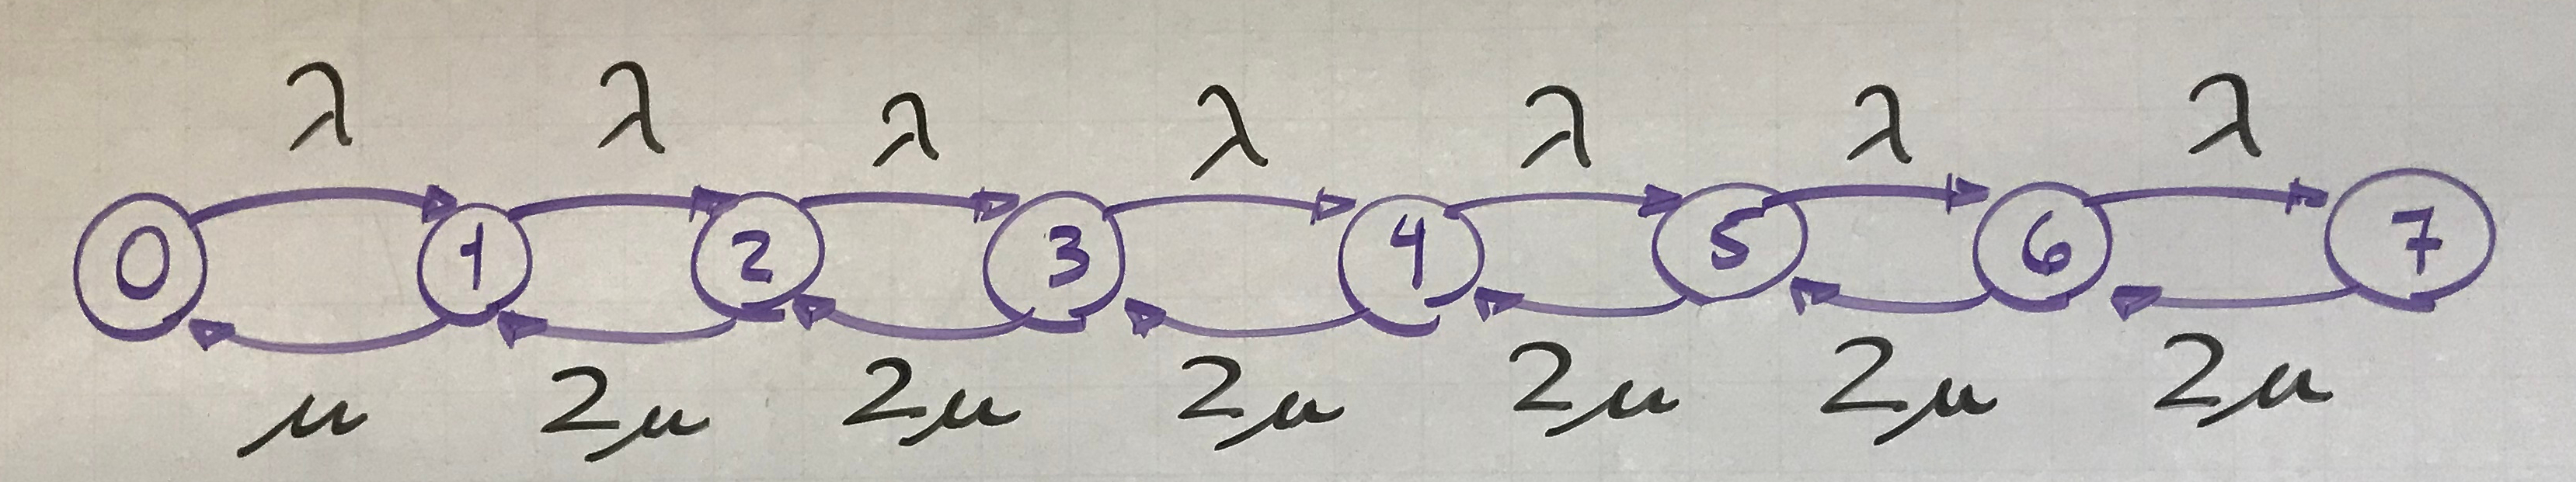
\includegraphics[width=0.8\textwidth]{problema-1-B.jpg}
\end{figure}

Para esta cadena, definiendo $\rho \define \lambda / ( 2 \mu )$, tenemos: 
\begin{align*}
& \lambda = 10 \quad \Longrightarrow \quad \rho = 0.250 \\
& \lambda = 15 \quad \Longrightarrow \quad \rho = 0.375 \\
& \lambda = 25 \quad \Longrightarrow \quad \rho = 0.625
\end{align*}
Las ecuaciones de balance son: 
\begin{align*}
& E_0 \; \colon \; \lambda \, \pi_0 \; = \; \mu \, \pi_1
\quad \Longrightarrow \quad
\pi_1 \; = \; 2 \, \rho \, \pi_0 \\
& E_1 \; \colon \; (\lambda + \mu) \, \pi_1
\; = \; \lambda \, \pi_0 + 2 \, \mu \, \pi_2
\quad \Longrightarrow \quad
\pi_2 \; = \; 2 \, \rho^2 \, \pi_0 \\
& E_2 \; \colon \; (\lambda + 2 \mu) \, \pi_2
\; = \; \lambda \, \pi_1 + 2 \, \mu \, \pi_3
\quad \Longrightarrow \quad
\pi_3 \; = \; 2 \, \rho^3 \, \pi_0 \\
& \vdots \\
& E_k \; \colon \; (\lambda + 2\mu) \, \pi_{k} \; = \; \lambda \, \pi_{k-1} + 2 \, \mu \, \pi_{k+1} \quad \Longrightarrow \quad
\pi_{k+1} \; = \; 2 \, \rho^{k+1} \, \pi_0 \\
& \vdots
\end{align*}
Ahora normalizamos para hallar la probabilidad del estado cero: 
\[
\pi_0 + 
2 \, \pi_0 \, \sum_{k=1}^7 \rho^k \; = \; 1 \quad \Longrightarrow \quad
\pi_0 \; = \; \left( 1 + 2 \, \sum_{k=1}^7 \rho^k \right)^{-1}
\]
Con esta probabilidad a la mano es f\'acil computar las siguienes, puesto que $\pi_1 = 2 \, \rho \, \pi_0$ y que para todo $k \geq 2$ es el caso que: 
\[
\pi_{k} \; = \; \rho \, \pi_{k-1}
\]
Consecuentemente: 
\begin{table}[htb]
\centering
\begin{tabular}{|c|c|c|c|}
\hline
\textbf{Estado} $\boldsymbol{i}$ & $\boldsymbol{\pi_i} \; ( \lambda = 10 )$ & $\boldsymbol{\pi_i} \; ( \lambda = 15 )$ & $\boldsymbol{\pi_i} \; ( \lambda = 25 )$ \\ \hline
0 & 0.600 & 0.455 & 0.238 \\ \hline
1 & 0.300 & 0.341 & 0.298 \\ \hline
2 & 0.075 & 0.128 & 0.186 \\ \hline
3 & 0.019 & 0.048 & 0.116 \\ \hline
4 & 0.005 & 0.018 & 0.073 \\ \hline
5 & 0.001 & 0.007 & 0.045 \\ \hline
6 & $\approx$0.000 & 0.003 & 0.028 \\ \hline
7 & $\approx$0.000 & 0.001 & 0.018 \\ \hline
\end{tabular}
\end{table}

\item \textbf{2 Puntos:} Para cada uno de los tres casos anteriores, eval\'ue si se cumplen o no los requisitos de la FAA. 

\emph{Soluci\'on:} Los requisitos de la FAA se traducen de la siguiente manera: 
\begin{itemize}
\item El primer requerimiento equivale a exigir que el n\'umero promedio de clientes en cola sea menor o igual a uno. \Iec
\[
\Exp[L_q] \; = \; \Exp[ \, \max \{ \, 0, X_t - 2 \} \, ]
\; = \; \sum_{k=0}^7 \, \pi_k \, \max \{ 0, k-2 \} \; \leq \; 1
\]
\item Como en este caso tenemos dos servidores, el segundo requerimiento exige que la probabilidad de que el estado del sistema sea menor o igual a seis debe ser mayor o igual al 95\%. \Iec
\[
\pi_0 + \pi_1 + \pi_2 + \pi_3 + \pi_4 + \pi_5 + \pi_6 \; \geq \; 0.95
\qquad
\Longleftrightarrow
\qquad
\pi_7 \; \leq \; 0.05
\]
\item El tercer requerimiento es igual al caso anterior, excepto que ahora la tasa de servicio efectia es de $2 \mu = 40$ aviones por hora. Con esta nueva tasa, tenemos: 
\begin{table}[H]
\centering
\begin{tabular}{|c|c|}
\hline
\textbf{Estado} $\boldsymbol{k}$ & \textbf{Probabilidad} $\boldsymbol{ \Pr( W_k \leq t)}$ \\ \hline
0 & 1  \\ \hline
1 & 1  \\ \hline
2 & $\approx$ 1.000 \\ \hline
3 & $\approx$ 1.000 \\ \hline
4 & $\approx$ 1.000 \\ \hline
5 & $\approx$ 1.000  \\ \hline
6 & $\approx$ 1.000  \\ \hline
7 & 0.9999  \\ \hline
\end{tabular}
\end{table}
N\'otese que sin importar el estado, la probabilidad de que el tiempo de espera no exceda el l\'imite siempre es mayor al 99\%. Consecuentemente, conclu\'imos que sin importar la tasa de arribo, el tercer requerimiento siempre se cumple. 
\end{itemize}

Ahora que entendemos los requerimientos en t\'erminos de teor\'ia de colas, analizamos el caso de cada tasa de arribo. 
\begin{itemize}
\item Para el caso cuando $\lambda = 10$ por hora, tenemos: 
\begin{align*}
& \Exp[L_q] \; = \; 0.032 < 1 \\
& \pi_7 \; = \; 0.000 < 0.05
\end{align*}
\item Para el caso cuando $\lambda = 15$ por hora, tenemos: 
\begin{align*}
& \Exp[L_q] \; = \; 0.122 < 1 \\
& \pi_7 \; = \; 0.001 < 0.05
\end{align*}
\item Para el caso cuando $\lambda = 25$ por hora, tenemos: 
\begin{align*}
& \Exp[L_q] \; = \; 0.599 < 1 \\
& \pi_7 \; = \; 0.018 < 0.05
\end{align*}
\end{itemize}
En conclusi\'on, con dos pistas de aterrizaje el aeropuerto satisface los requerimientos de la FAA sin importar la tasa de arribo. 

\end{enumerate}

\end{problem}
\fullskip

% -----------------------------------------------------------------
\begin{problem}
\textbf{[8 Puntos]} El lunes, cierta acci\'on cerr\'o a 10 d\'olares. El martes se espera que la acci\'on cierre a 9, 10 u 11 d\'olares, con probabilidades respectivas de 0.3, 0.3 y 0.4. El mi\'ercoles, \linebreak se espera que la acci\'on cierre 10\% abajo, sin cambio o 10\% arriba del cierre del martes, con las siguientes probabilidades: 

\begin{figure}[htb]
\centering
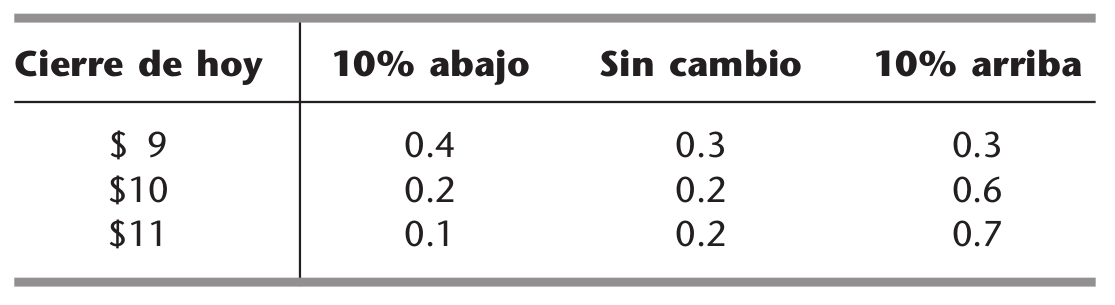
\includegraphics[width=0.6\textwidth]{problema-acciones.jpg}
\end{figure}

El martes recibe instrucciones de comprar 100 acciones antes del jueves. Todas las compras se hacen al final del d\'ia, al precio de cierre conocido de ese d\'ia, de manera que sus \'unicas opciones son comprar al final del martes o al final del mi\'ercoles. Usted quiere determinar una estrategia \'optima: comprar el martes o aplazar la compra hasta el mi\'ercoles, dado el precio al cierre del martes, con el fin de minimizar el precio esperado de compra. Desarrolle y eval\'ue un \'arbol de decisi\'on para determinar la estrategia \'optima. 

\emph{Clarificaci\'on:} Si usted entendi\'o que la decisi\'on de comprar el martes o el mi\'ercoles debe ser tomada de antemano, por favor siga la Soluci\'on A. En cambio, si usted entendi\'o, correctamente, que se puede tomar una decisi\'on el martes dependiendo del precio de la acci\'on al cierre de ese d\'ia, por favor siga la Soluci\'on B. 

\emph{Soluci\'on A:} En este problema nuestro objetivo es minimizar el costo de compra de las acciones, \ie buscamos comprarlas al menor precio posible. Para esto, primero supongamos que se decide de antemano realizar la compra el martes. Entonces el precio esperado es: 
\[
(\$9)(0.3) + (\$10)(0.3) + (\$11)(0.4) \; = \; \$10.10
\]
Consecuentemente, el costo esperado de la compra ser\'ia de \$1010. En cambio, si se decide de antemano hacer la compra el mi\'ercoles, el \'arbol de probabilidad de precios de de cierre es como se muestra en la siguiente fotograf\'ia. 

\begin{figure}[H]
\centering
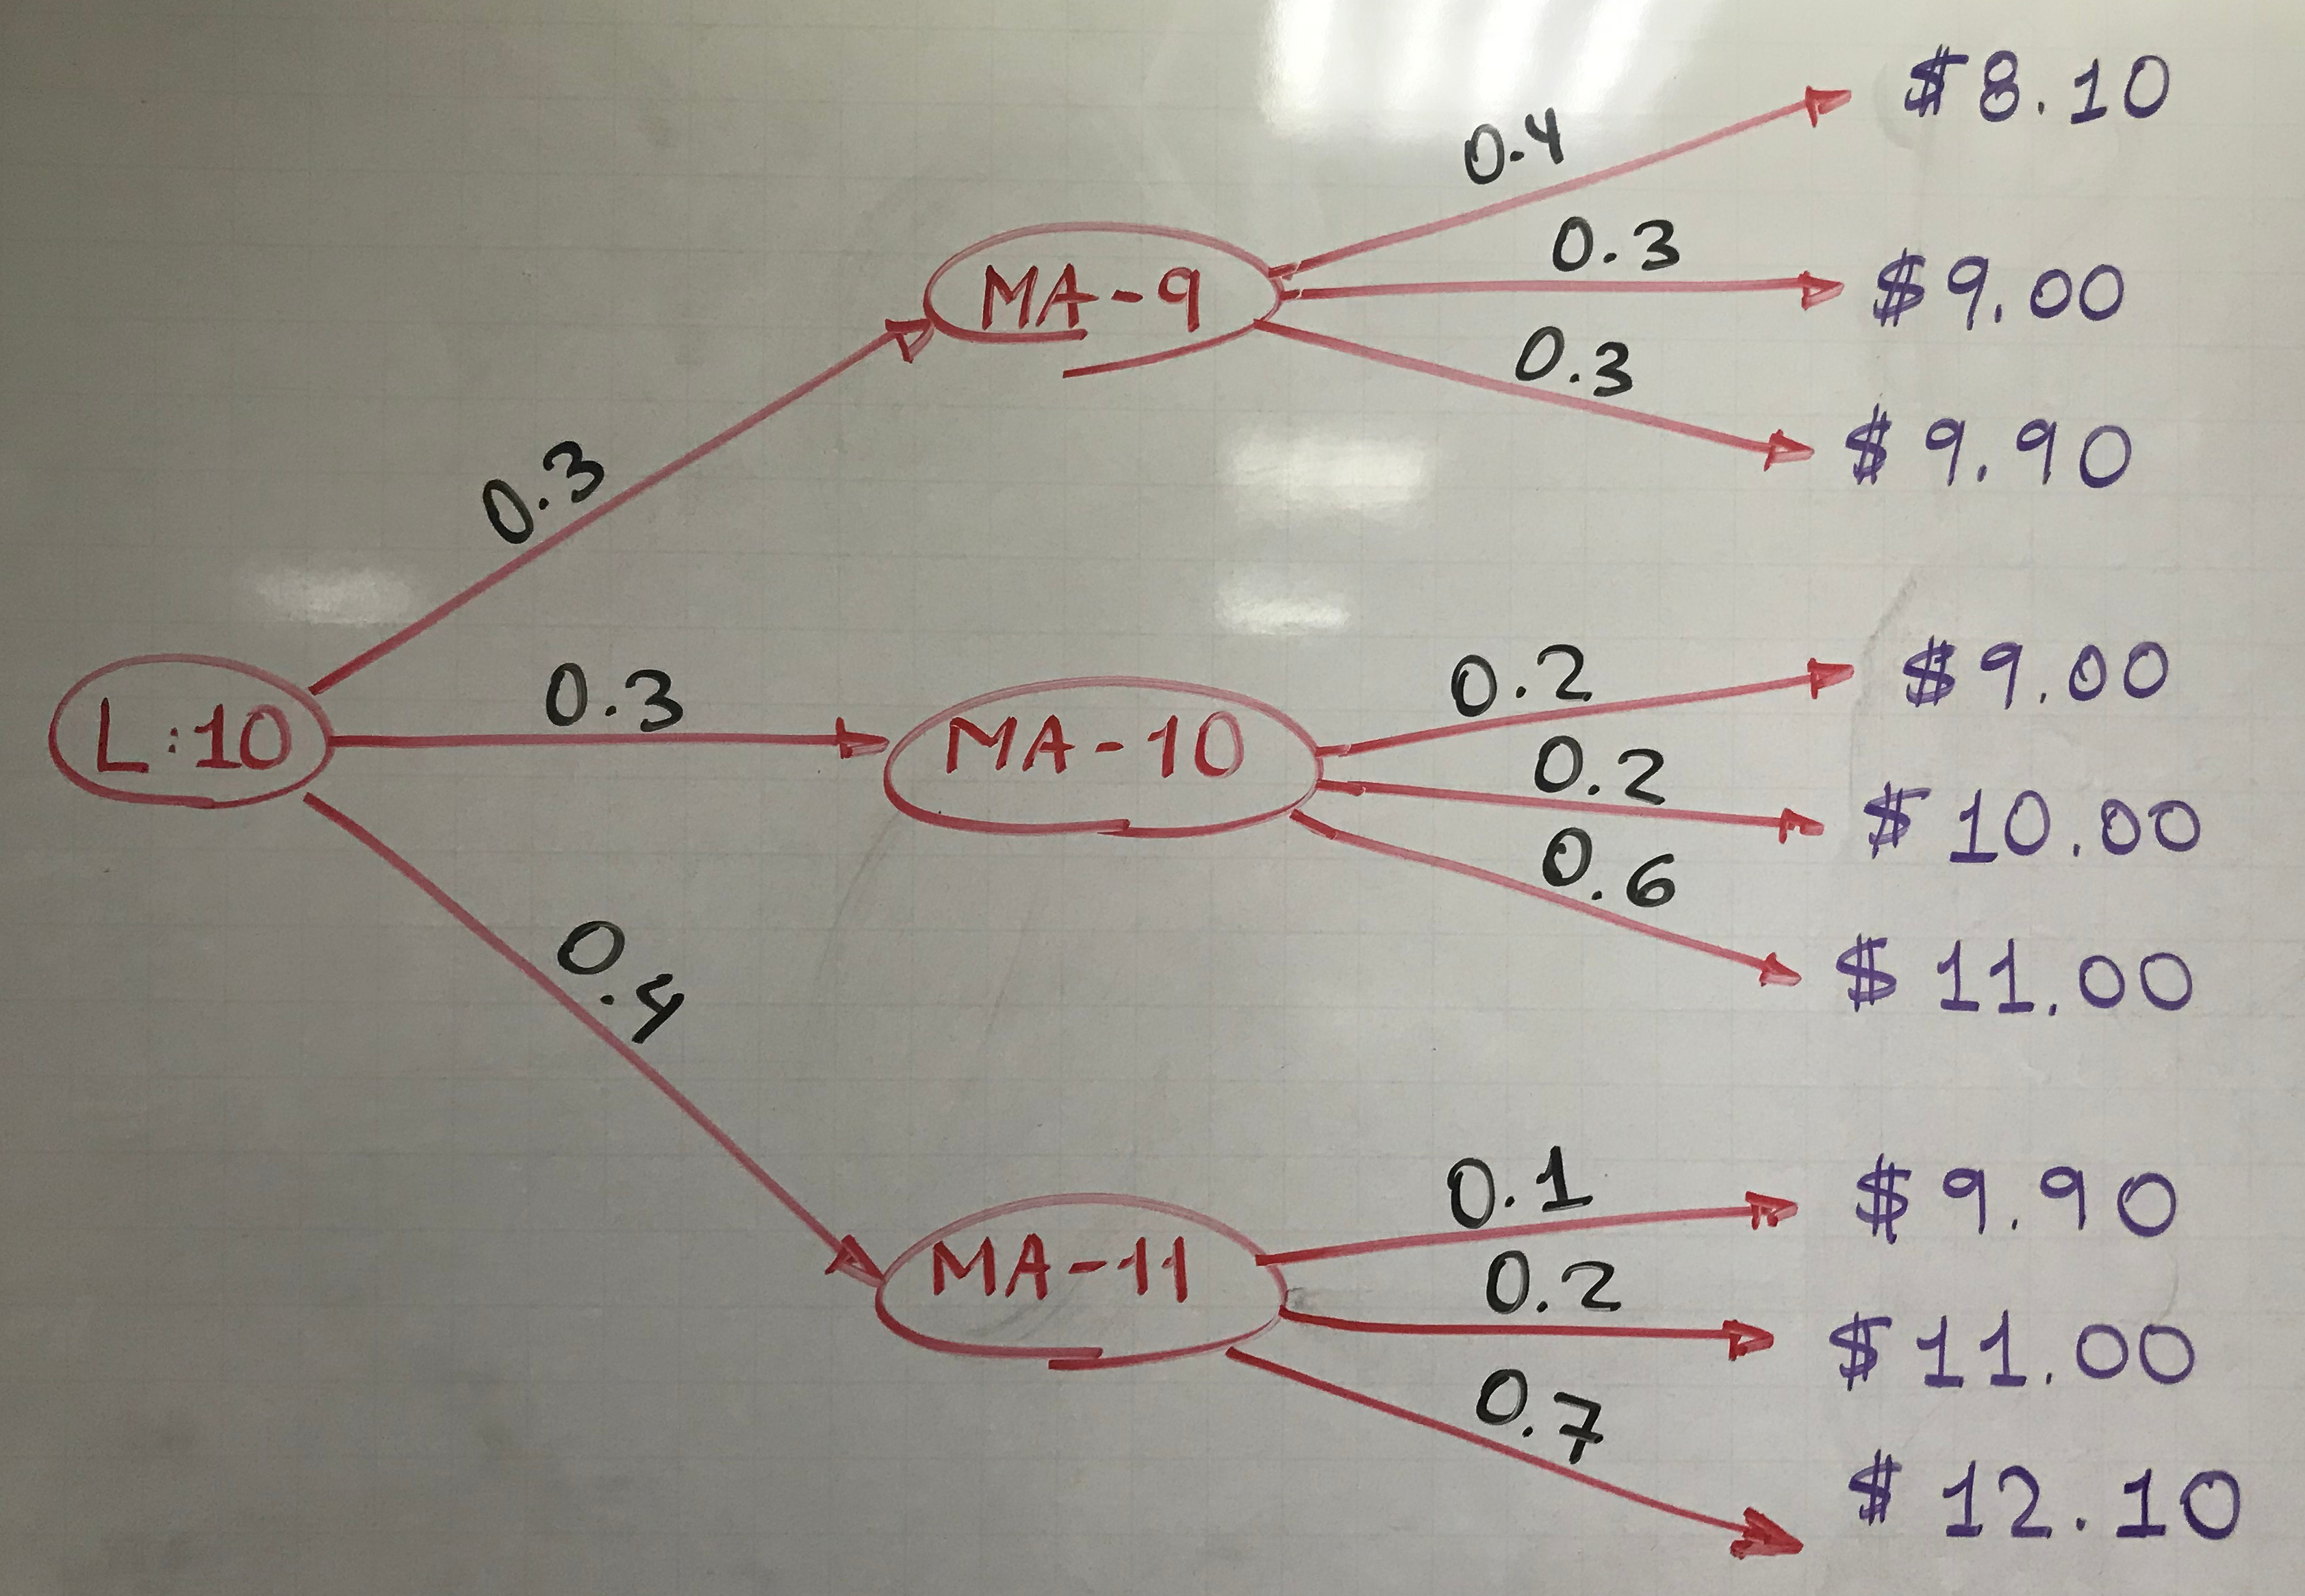
\includegraphics[width=0.72\textwidth]{problema-2.jpg}
\end{figure}

Podamos el \'arbol calculando los costos esperados en los nodos MA-9, MA-10 y MA-11. 
\begin{align*}
& \Exp[\text{MA-9}] \; = \; 
(\$8.10)(0.4) + (\$9.00)(0.3) + (\$9.90)(0.3)
\; = \; \$8.91 \\
& \Exp[\text{MA-10}] \; = \; 
(\$9.00)(0.2) + (\$10.00)(0.2) + (\$11.00)(0.6)
\; = \; 10.40 \\
& \Exp[\text{MA-11}] \; = \; 
(\$9.90)(0.1) + (\$11.0)(0.2) + (\$12.10)(0.7) \; = \; \$11.66
\end{align*}
Finalmente, calculamos el costo esperado del nodo L-10. 
\[
\Exp[\text{L-10}] \; = \;
(\$8.91)(0.3) + (\$10.40)(0.3) + (\$11.66)(0.4) \; = \; \$10.46
\]
Vemos as\'i que el costo esperado de la compra en este caso ser\'ia de \$1046, \ie \$36 m\'as de lo que costar\'ia comprarla el martes. Conclu\'imos as\'i que la estrategia \'optima es comprar las acciones el martes. 

\emph{Soluci\'on B:} Nuevamente, si se decide de antemano que se va a realizar la compra el d\'ia martes, el precio esperado es: 
\[
(\$9)(0.3) + (\$10)(0.3) + (\$11)(0.4) \; = \; \$10.10
\]
Consecuentemente, el costo esperado de la compra ser\'ia de \$1010. En cambio, considerando cada uno de los posibles precios de cierre del martes, vemos que: 
\begin{itemize}
\item Si el precio es de \$9.00 entonces estamos en el nodo MA-9, cuyo precio esperado de cierre el mi\'ercoles es de \$8.91, tal como se calcul\'o anteriormente. En este caso la acci\'on \'optima es esperar hasta el mi\'ercoles. 
\item Si el precio es de \$10.00 entonces estamos en el nodo MA-10, cuyo precio esperado de cierre el mi\'ercoles es de \$10.40. En este caso la acci\'on \'optima es comprar la acci\'on el mismo martes al precio de \$10.00. 
\item Si el precio es de \$11.00 entonces estamos en el nodo MA-11, cuyo precio esperado de cierre el mi\'ercoles es de \$11.66. En este caso la acci\'on \'optima es comprar la acci\'on el mismo martes al precio de \$11.00. 
\end{itemize}
De esta manera, el precio esperado de compra es: 
\[
(\$8.91)(0.3) + (\$10.00)(0.3) + (\$11.00)(0.4) \; = \; \$10.07
\]
Vemos as\'i que el costo esperado de la compra en este caso ser\'ia de \$1007, \ie \$3 menos de lo que costar\'ia comprarla el martes sin considerar el precio de cierre. Conclu\'imos as\'i que la estrategia \'optima es: 
\begin{itemize}
\item Si el precio de cierre del martes es de \$9.00, esperar hasta el mi\'ercoles para comprar. 
\item Caso contarrio, \ie si el precio de cierre del martes es de \$10.00 u \$11.00, comprar el mismo martes. 
\end{itemize}


\end{problem}
\fullskip

\end{document}
